\documentclass[dvipdfm, t]{beamer}
% \usepackage{amsmath}
\usepackage{bm}
\usepackage{txfonts}
% \usepackage{graphicx}
% \usepackage{hyperref}
% \usepackage{url}

%条件付き独立でない、という記号
\newcommand{\nPerp}{\Perp\hspace{-.95em}/}

%%ナビゲーションシンボルを表示しない
%%dvipdfmでは動かないため
\setbeamertemplate{navigation symbols}{}

\renewcommand{\kanjifamilydefault}{\gtdefault} % 和文既定をゴシックに変更

\title{PRML\_titech 8.1 - 8.2}
\author{榊原隆文(@saka\_bar)}
% \date{February 26, 2015}
\date{\today}

\setbeamertemplate{footline}[frame number]
\setbeamerfont{footline}{size=\small,series=\bfseries}
\setbeamercolor{footline}{fg=black,bg=black}

%数式をTeXの元々のフォントにする
\usefonttheme{professionalfonts}

\begin{document}
\maketitle

 \section*{自己紹介}
 \begin{frame}{自己紹介(前回とほぼ変化なし)}
 \begin{tabular}[tb]{cc}

  \begin{minipage}{0.7\hsize}
   \begin{center}
    \begin{itemize}
     \item 榊原隆文 (twitter:@saka\_bar さかばー)
     \item すずかけ台の奥村研に所属
           \begin{itemize}
            \item 専門は自然言語処理
                  \begin{itemize}
                   \item テキスト集合からの知識獲得
                  \end{itemize}
           \end{itemize}
     \item 好きなもの
           \begin{itemize}
            \item 唐揚げ
            \item 凌駕
            \item Haskell
            \item IIDX DP
            \item 漢直(漢字直接入力)
                  \begin{itemize}
                   \item 紹介スライド
                  \end{itemize}

                  \href{http://www.slideshare.net/takafumisakakibara75/tutcode}{\structure{http://www.slideshare.net/takafumisakakibara75/tutcode}}
           \end{itemize}
    \end{itemize}
   \end{center}
  \end{minipage}

  \begin{minipage}{0.3\hsize}
   \begin{center}
    \begin{figure}[htbp]
     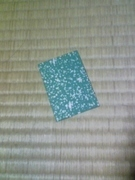
\includegraphics[bb=0 0 135 180,scale=0.5]{./figure/icon.jpg}
    \end{figure}
   \end{center}
  \end{minipage}

 \end{tabular}
\end{frame}

\begin{frame}{このスライドの特徴(前回とほぼ変化なし)}
 \begin{itemize}
  \item スライド作成のために\LaTeX のBeamerパッケージを利用
        \begin{itemize}
         \item PowerPointを使いたくない
         \item 前の発表の時にBeamerで痛い目見たけど、今回は大丈夫だろうか…
        \end{itemize}
  \item gitでバージョン管理
        % \begin{itemize}
  %  \item このスライドはタグのv0.1と対応
          % \end{itemize}
  \item ソースをgithubで公開
        % \begin{itemize}
  % \item \href{https://github.com/sakabar/prml_titech_2-3-1_2-3-7}{\structure{\url{https://github.com/sakabar/prml_titech_2-3-1_2-3-7}}}
          % \end{itemize}
  \item PDFをSlideShareで公開
        % \begin{itemize}
  %  \item \href{http://www.slideshare.net/takafumisakakibara75/slide-41820194}{\structure{\url{http://www.slideshare.net/takafumisakakibara75/slide-41820194}}}
          % \end{itemize}
 \end{itemize}
\end{frame}


 \begin{frame}{もくじ}
  \tableofcontents
 \end{frame}

 \section{8.1 ベイジアンネットワーク}
 %currentsectionオプションを指定することで、現在のセクションのみを強調表示することができる
 \begin{frame}{もくじ}
  \tableofcontents[currentsection]
 \end{frame}
 \begin{frame}{この章の気持ち}
 \begin{itemize}
  \item 確率論は2つの単純な等式から成り立っている
        \begin{itemize}
         \item 加法定理
         \item 乗法定理
               %TODO 加法定理と乗法定理の式を載せる
        \end{itemize}
  \item → どんなに複雑な確率的推論・学習方法も、これらによって分解することができる
  \item そこでグラフィカルモデルですよ
        \begin{enumerate}
         \item 確率モデル構造を視覚化できるので、新しいモデルの設計方針を決めるのに役立つ
         \item グラフの構造を調べることにより、条件付き独立性(8.2章)などのモデルの性質に関する知見が得られる
         \item 学習や推論のための計算をグラフ上の操作として表現できる
        \end{enumerate}
 \end{itemize}
\end{frame}

\begin{frame}{ことば}
 %TODO 分かりやすい図の挿入
 \begin{itemize}
  \item リンク
  \item ノード
  \item ベイジアンネットワーク(有向グラフィカルモデル)
  \item マルコフ確率場(無向グラフィカルモデル)
 \end{itemize}
\end{frame}

\begin{frame}{ベイジアンネットワーク}
 \begin{itemize}
  \item グラフィカルモデル: 広い確率分布のクラスをグラフで記述できる
 \end{itemize}
 \begin{eqnarray*}
  p(a,b,c) &=& p(c|a,b)p(a,b) \\
  & =& p(c|a,b)p(b|a)p(a)
 \end{eqnarray*}
 \begin{itemize}
  \item このような分解は、任意の同時分布に対して常に可能
  \item 左辺は$a,b,c$対称だが、右辺は対称でないことに注意
 \end{itemize}
 %TODO 親ノード、子ノード、図の追加
\end{frame}

\begin{frame}{$K$変数の場合}
 % \begin{itemize}
 %  \item $K$変数の同時分布$p(x_1,...x_K)$の場合を考える
   % \end{itemize}
 \begin{eqnarray}
  p(x_1,...,x_K) = p(x_K|x_1,...,x_{K-1})\dots p(x_2|x_1)p(x_1)\label{164842_7Feb15}
 \end{eqnarray}
 \begin{itemize}
  \item $K$の値を決めれば、この同時分布は$K$個のノードを持つ有向グラフとして表現される
  \item 各ノードは式(\ref{164842_7Feb15})の右辺の因子のうちの1つの条件付き分布に対応
  \item 各ノードは自分よりも小さい番号が振られたすべてのノードから向かってくるリンクを持つ
  \item 全結合
  \item グラフはリンクが存在しないことを通して、分布のクラスに関する情報を表現する
 \end{itemize}
 %TODO K変数のときの図?
\end{frame}

\begin{frame}{同時確率分布を条件付き分布の積で表す}
 %TODO 図8.2の挿入
 \begin{itemize}
  \item 例
 \end{itemize}
 \begin{eqnarray*}
  p(x_1)p(x_2)p(x_3)p(x_4|x_1,x_2,x_3)p(x_5|x_1,x_3)p(x_6)p(x_4)p(x_7|x_4,x_5)
 \end{eqnarray*}
 \begin{itemize}
  \item $K$個のノードを持つグラフに対応する同時分布は次の式で与えられる。ここで、$pa_k$は$x_k$の親ノード集合
 \end{itemize}
 \begin{eqnarray*}
  p(\bm{x}) = \prod_{k=1}^{K}p(x_k|pa_k)
 \end{eqnarray*}
\end{frame}

\begin{frame}{説明}
 % \begin{eqnarray*}
 %  p(\bm{x}) = \prod_{k=1}^{K}p(x_k|pa_k)
   % \end{eqnarray*}
 \begin{itemize}
  \item この等式は、与えられた有向グラフィカルモデルに対応する同時分布の分解特性を表現
  \item 各ノードは1つの変数だけでなく、変数集合やベクトル値変数を表現させることも可
  \item ここでの有向グラフは有向閉路を持たないという制約を満たす(有向非循環グラフ, DAG)
  \item 有向閉路を持たないことと、大きい番号を持つノードから小さい番号を持つノードへのリンクが存在しないへのリンクが存在しないようにノードを順序付けられることは等価(演習8.2)
        \begin{itemize}
         \item → 次スライドで軽く説明
        \end{itemize}
 \end{itemize}
 %TODO 演8.1,8.2を解いてスライドに入れる
 %TODO 菅原さんの資料を確認すること
\end{frame}

\begin{frame}{演習8.2 解}
 \begin{itemize}
  \item 問: 「有向グラフにおいて、すべてのノードについて、自分より小さい番号を持つノードに向かうリンクが存在しないようにノードを順序を付けることができるなら、有向閉路は存在しない」ことを示せ
  \item 対偶をとると、「有向グラフにおいて有向閉路が存在するならば、あるのノードについて、自分より小さい番号を持つノードに向かうリンクが存在するようにノードを順序を付けられている」
  \item 有向閉路に注目すると、初めのノードに戻ってくるときに「自分より小さい番号を持つノードに向かうリンク」を通ることになる
  % \item 有向閉路は「あるノードから出発して矢印に従って進んだ後、また初めのノードに戻ってくるような閉じた経路」
 \end{itemize}
\end{frame}


 \section{8.1.1 例:多項式曲線フィッティング}
 \begin{frame}{もくじ}
  \tableofcontents[currentsection]
 \end{frame}
 \begin{frame}{8.1.1 例: 多項式曲線フィッティング}
 \begin{itemize}
  \item 1.2.6節で紹介したベイズ多項式回帰モデルをグラフィカルモデルで表すと、図のようになる
        %TODO 図8.3の挿入
  \item ここで、複数のノードをコンパクトに表現するために、\alert{プレート}を導入する
        %TODO 図8.4の挿入
 \end{itemize}
\end{frame}

\begin{frame}{決定的パラメータ・観測変数・潜在変数}
 \begin{itemize}
  \item 確率的な変数と同様に、モデルのパラメータも陽に書いた方が便利な場合もある
  \item 値が確定しているパラメータに関するノードは小さな塗りつぶされた円で表現する
  \item 機械学習やパターン認識問題では、多くの場合、確率変数のうちいくつかを特定の観測値に対応させる。観測した確率変数は、グラフ上では塗りつぶされた円で表現する
  \item 一方、観測されていないノードを潜在変数と呼ぶ
 \end{itemize}
\end{frame}

\begin{frame}{複雑な例}
 \begin{eqnarray*}
  p(\hat{t}, \bm{t}, w| \hat{x}, \bm{x}, \alpha , \sigma^2) = \left[\prod_{n=1}^{N}p(t_n|x_n, \bm{w}, \sigma^2)\right]p(\bm{w}|\alpha)p(\hat{t}|\hat{x}, \bm{w}, \sigma^2)
 \end{eqnarray*}
 %TODO 図8.7の挿入
 \begin{itemize}
  \item グラフィカルモデルと見くらべると、たしかに依存関係を簡潔に表すことができている
  \item ただし、モデルの具体的な中身は、式を見ないとわからない
 \end{itemize}
\end{frame}


 \section{8.1.2 生成モデル}
 \begin{frame}{もくじ}
  \tableofcontents[currentsection]
 \end{frame}
 \begin{frame}{伝承サンプリング}
 \begin{itemize}
  \item 与えられた確率分布に対して、それに従うサンプルを発表させたい場合が多くある
        \begin{itemize}
         \item サンプリング法については11章
         \item ここでは、伝承サンプリングのみ紹介
        \end{itemize}
  \item 伝承サンプリングとは、番号の最も小さいノードから順にサンプルを発生させていき、最終的に同時分布$p(\bm{x})$を求める方法である
 \end{itemize}
 %TODO 図8.2を再び挿入して説明?
\end{frame}

\begin{frame}{生成モデル}
 \begin{itemize}
  \item 確率モデルの実際のアプリケーションでは、通常グラフの末端ノードに対応する大きい番号が振られた変数が観測値を表し、小さい番号が振られたノードが潜在変数に対応する
  \item このようなモデルが観測データを発生する過程を表現していると解釈することもできる
 \end{itemize}
\end{frame}

\begin{frame}{生成モデルの例: 物体認識問題}
 \begin{itemize}
  \item この問題では、物体の像が各観測データ点に対応し、この観測データから物体の種類を推論することが目的
  \item この問題では、例えば物体の位置・向きを隠れ変数とみなすことができる
  \item このグラフィカルモデルでは、全てのノードに関して確率分布が与えられているため、「架空」のデータを発生させることができる。
        \begin{itemize}
         \item このようなモデルを\alert{生成モデル}と呼ぶ
        \end{itemize}
 \end{itemize}
 %TODO 図8.8の挿入
\end{frame}


 \section{8.1.3 離散変数}
 \begin{frame}{もくじ}
  \tableofcontents[currentsection]
 \end{frame}
 \begin{frame}{離散変数}
 \begin{itemize}
  \item 指数型分布族(2.4節)は複雑な確率分布を構築するための基本構成要素として利用される
  \item グラフィカルモデルは、これらの構成要素がどのように接続されているかを表現するための便利な枠組みを提供する
  \item 有向グラフの親子対が共役関係(同じような分布)になるように分布を選べば、そのモデルは非常に良い性質を持つ
        \begin{itemize}
         \item 特に親ノードと子ノードが共に\alert{離散変数}
         \item または、親ノードと子ノードが共に\alert{ガウス変数}
        \end{itemize}
 \end{itemize}
\end{frame}

\begin{frame}{離散変数}
 \begin{itemize}
  \item $K$状態離散変数$x$を1-of-$K$表現を用いて表現する
  \item 確率分布$p(\bm{x}|\bm{\mu})$は
 \end{itemize}
 \begin{eqnarray*}
  p(\bm{x}|\bm{\mu}) = \prod_{k=1}^{K}\mu_k^{x_k}
 \end{eqnarray*}
 で与えられ、パラメータ$\bm{\mu}=(\mu_1,...,\mu_K)^{\mathrm{T}}$によって支配される
 \begin{itemize}
  \item 次に、2つの$K$状態離散変数$x_1,x_2$があるとし、これらの同時分布をモデル化することを考える
 \end{itemize}
 \begin{eqnarray*}
  p(\bm{x_1},\bm{x_2}|\mu) = \prod_{k=1}^{K}\prod_{l=1}^{K}\mu_{kl}^{x_{1k}x_{2l}}
 \end{eqnarray*}
 \begin{itemize}
  \item この分布は$K^2-1$個のパラメータに支配される
  \item 変数が2でなく$M$個のときは、$K^M-1$個のパラメータ
        \begin{itemize}
         \item \structure{指数オーダーorz}
        \end{itemize}
 \end{itemize}
\end{frame}

\begin{frame}{リンクを仮定した時(いるか?)}
 \begin{itemize}
  \item %TODO 乗法定理を使った部分入れるか?
  % \item 同時分布を$p(\bm{x_1},\bm{x_2}) = p(\bm{x_2}| \bm{x_1})p(\bm{x_1})$の形に因数分解すると、パラメータの総数は
 \end{itemize}
\end{frame}

\begin{frame}{どうするのか?}
 \begin{itemize}
  \item グラフに制約を加えることで、パラメータ数を減らす
  \item 変数$\bm{x_1}, \bm{x_2}$が独立であると仮定すると、全パラメータ数は$2(K-1)$である
        \begin{itemize}
         \item この場合、$\bm{x_1}$と$\bm{x_2}$を結ぶリンクが除去されたことになる
        \end{itemize}
  \item 一般に、$M$個の独立な$K$状態離散変数上の分布の場合、全パラメータ数は$M(K-1)$
        \begin{itemize}
         \item \alert{線形オーダになった!}
        \end{itemize}
  \item ただし、この操作によって表現可能な分布のクラスは制限される
 \end{itemize}
\end{frame}

\begin{frame}{チェイン}
 \begin{itemize}
  \item %TODO 図8.10の挿入
 \end{itemize}
\end{frame}

\begin{frame}{パラメータの共有(結合)}
 \begin{itemize}
  \item %TODO 図8.11と図8.12の挿入
 \end{itemize}
\end{frame}

\begin{frame}{パラメトリックモデルの利用}
 \begin{itemize}
  \item %TODO 式8.10あたりか?
 \end{itemize}
\end{frame}



 \section{8.1.4 線形ガウスモデル}
 \begin{frame}{もくじ}
  \tableofcontents[currentsection]
 \end{frame}
 \begin{frame}{線形ガウスモデル}
 \begin{itemize}
  \item この節では、要素変数上の線形ガウスモデルに対応する有向グラフによって、多変量ガウス分布を表現する方法を示す
  \item 対角共分散を持つガウス分布と一般のガウス分布とを両極端とするような興味ある構造を分布に持たせる
  \item 線形ガウスモデルの利用例
        \begin{itemize}
         \item 確率主成分分析
         \item 因子分析
         \item 線形動的システム
        \end{itemize}
 \end{itemize}
\end{frame}

\begin{frame}{同時分布}
 \begin{itemize}
  \item $D$個の変数上の任意の有向非循環グラフを考える
  \item 線形ガウスモデルでは、分布の平均はノード$i$の親ノード$pa_i$状態の線形結合
        \begin{eqnarray*}
         p(x_i|pa_i) = \mathcal{N} \left(x_i \sum_{j \in pa_i}w_{ij}x_j + b_i, v_i \right)
        \end{eqnarray*}
  \item 同時分布の対数は、グラフに含まれるすべてのノード上の条件付き分布の積の対数
        \begin{eqnarray*}
         \ln p(\bm{x}) &=& \sum_{i=1}^{D}\ln p(x_i | pa_i)\\
         &= & -\sum_{i=1}^{D}\frac{1}{2v_i}(x_i - \sum_{j \in pa_i}w_{ij}x_j-b_i)^2 + \mathrm{const}
        \end{eqnarray*}
  \item この式は$\mathrm{x}$の成分に関する2次関数→\alert{同時分布$p(\mathrm{x})$は多変量ガウス分布}
 \end{itemize}
\end{frame}

\begin{frame}{平均と分散}
 \begin{itemize}
  \item この同時分布の平均と分散は再帰的に決められる
  \item 各変数$x_i$は以下のように書ける
        \begin{eqnarray*}
         x_i = \sum_{j \in pa_i}w_{ij}x_j + b_i + \sqrt{v_i}\epsilon_i
        \end{eqnarray*}
  \item この期待値を取ると
        \begin{eqnarray*}
         \mathbb{E}[x_i] = \sum_{j \in pa_i}w_ij\mathbb{E}[x_j]+b_i
        \end{eqnarray*}
  \item この式をグラフ上の最も小さいノードから順番に再帰的に計算することで、$\mathbb{E}[\mathrm[x]]=(\mathbb{E}[x_1], ... , \mathbb{E}[x_D])^{\mathrm{T}}$の全成分の値が得られる
 \end{itemize}
\end{frame}

\begin{frame}{共分散}
 \begin{itemize}
  \item 求めた$\mathbb{E}[x_i]$を利用する
 \end{itemize}
 \begin{eqnarray*}
  x_i = \sum_{j \in pa_i}w_{ij}x_j + b_i + \sqrt{v_i}\epsilon_i
 \end{eqnarray*}
 \begin{eqnarray*}
  \mathbb{E}[x_i] = \sum_{j \in pa_i}w_{ij}\mathbb{E}[x_j]+b_i
 \end{eqnarray*}
 \begin{eqnarray*}
  \mathrm{cov}[x_i, x_j] &=& \mathbb{E}[(x_i-\mathbb{E}[x_i])(x_j-\mathbb{E}[x_j])]\\
  &= & \mathbb{E}\left[(x_i-\mathbb{E}[x_i])\left\{\sum_{k \in pa_j}w_{jk}(x_k-\mathbb{E}[x_k])+\sqrt{v_j}\epsilon_j \right\}\right]\\
  &= & \sum_{k \in pa_j}w_{jk}\mathrm{cov}[x_i,x_k]+I_{ij}v_j
 \end{eqnarray*}
\end{frame}


 \section{8.2 条件付き独立性}
 \begin{frame}{もくじ}
  \tableofcontents[currentsection]
 \end{frame}
 \begin{frame}{$B>r7oIU$-FHN)@-(B}
 \begin{itemize}
  \item 3$BJQ?t(B$a,b,c$$B$KBP$7!"(B$b$$B$*$h$S(B$c$$B$,M?$($i$l$?$H$-!"(B$a$$B$N>r7oIU$-J,I[$,(B$b$$B$NCM$K0MB8$7$J$$$H$9$k!#$9$J$o$A!"(B
 \end{itemize}
 \begin{eqnarray*}
  p(a|b,c) = p(a|c)
 \end{eqnarray*}
 \begin{itemize}
  \item $B$3$N$H$-!"(B$c$$B$,M?$($i$l$?2<$G!"(B$a$$B$O(B$b$$B$KBP$7$F>r7oIU$-FHN)$G$"$k(B

  \item $c$$B$G>r7oIU$1$i$l$?(B$a$$B$*$h$S(B$b$$B$NF1;~J,I[$K$D$$$F9M$($k$H!">r7oIU$-FHN)@-$O<!$N$h$&$KI=8=$5$l$k(B
 \end{itemize}
 \begin{eqnarray*}
  p(a,b|c) &=& p(a|b,c)p(b|c)\\
  &= & p(a|c)p(b|c)
 \end{eqnarray*}
\end{frame}

\begin{frame}{$BCm0U(B}
 \begin{itemize}
  \item $B>r7oIU$-FHN)@-$NDj5A$O!"(B$c$$B$,$"$kFCDj$NCM$r$H$C$?$H$-$@$1$G$J$/!"(B$c$$B$N<h$jF@$k$9$Y$F$N2DG=$JCM$KBP$7$FA0=R$N<0$,@.$jN)$D$3$H$G$"$k(B
  \item $B>r7o$-FHN)$O<!$N$h$&$KI=$9$3$H$b$"$k(B
        \begin{eqnarray*}
         a \Perp b \ | \ c
        \end{eqnarray*}
        \begin{itemize}
         \item $c$$B$,M?$($i$l$?$H$-!"(B$a$$B$,(B$b$$B$KBP$7$F>r7oIU$-FHN)(B
        \end{itemize}
  % \item %TODO P85$B$N@bL@$rF~$l$k(B?
 \end{itemize}
\end{frame}


 \section{8.2.1 3つのグラフの例}
 \begin{frame}{もくじ}
  \tableofcontents[currentsection]
 \end{frame}
 \begin{frame}{3つのグラフの例}
 \begin{itemize}
  \item 有向グラフの条件付き独立性を考えるため、ノードを3つだけ持つ簡単な3種類のグラフについて考える
        \begin{itemize}
         \item tail-to-tail 型

               \includegraphics[width=4cm]{./figure/Figure8.15.eps}

         \item head-to-tail 型

               \includegraphics[width=4cm]{./figure/Figure8.17.eps}

         \item head-to-head 型

               \includegraphics[width=4cm]{./figure/Figure8.19.eps}

        \end{itemize}
 \end{itemize}
\end{frame}

\begin{frame}{tail-to-tail型}
 \begin{center}
  \includegraphics[width=4cm]{./figure/Figure8.15.eps}
 \end{center}
 \begin{itemize}
  \item このグラフに対応する同時分布は以下の式で表される
        \begin{eqnarray*}
         p(a,b,c) = p(a|c)p(b|c)p(c)
        \end{eqnarray*}
  \item どの変数も観測されていないとすると、$a$と$b$が独立かどうかは両辺を$c$に関して周辺化すれば調べられる
        \begin{eqnarray*}
         p(a,b) = \sum_c p(a|c)p(b|c)p(c)
        \end{eqnarray*}
  \item この式は一般には積$p(a)p(b)$には分解できないので、
        \begin{eqnarray*}
         a \nPerp\ b \ | \ \emptyset
        \end{eqnarray*}
 \end{itemize}
\end{frame}

\begin{frame}{tail-to-tail型}
 \begin{center}
  \includegraphics[width=4cm]{./figure/Figure8.15.eps}
 \end{center}
 \begin{itemize}
  \item 一方、変数$c$で条件付けてみると、
        \begin{eqnarray*}
         p(a,b|c) &=& \frac{p(a,b,c)}{p(c)}\\
         &= & p(a|c)p(b|c)
        \end{eqnarray*}
        これより、条件付き独立性
        \begin{eqnarray*}
         a \Perp b \ | \ c
        \end{eqnarray*}
        が導出された
  % \item ノード$c$を経由する、ノード$a$からノード$b$までの経路を考えれば、この結果をグラフ上で簡潔に説明できる。
  % \item ノード$c$はこの経路に関して\alert{tail-to-tail}であると言われる
  % \item ノード$a$と$b$とを結ぶこのような経路が存在すると$a$と$b$は独立にはならない。しかし、図のようにノード$c$に関して条件付ければ、この条件付きノードは$a$から$b$への経路を遮断して$a$と$b$とを(条件付き)独立にする
 \end{itemize}
\end{frame}

\begin{frame}{head-to-tail型}
 \begin{center}
  \includegraphics[width=4cm]{./figure/Figure8.17.eps}
 \end{center}
 \begin{eqnarray*}
  p(a,b,c) = p(a)p(c|a)p(b|c)
 \end{eqnarray*}
 \begin{itemize}
  \item まず、$c$に関して周辺化することにより$a$と$b$の独立性を調べる
        \begin{eqnarray*}
         p(a,b) = p(a)\sum_c p(c|a)p(b|c) = p(a)p(b|a)
        \end{eqnarray*}
        この式は一般に$p(a)p(b)$の形に因数分解できないため、前の例と同様に
        \begin{eqnarray*}
         a \nPerp \ b | \emptyset
        \end{eqnarray*}
        が言える
 \end{itemize}
\end{frame}

\begin{frame}{head-to-tail型}
 \begin{center}
  \includegraphics[width=4cm]{./figure/Figure8.17.eps}
 \end{center}
 \begin{itemize}
  \item 次に、ノード$c$で条件付けると
        \begin{eqnarray*}
         p(a,b|c) &=& \frac{p(a,b,c)}{p(c)}\\
         & =& \frac{p(a)p(c|a)p(b|c)}{p(c)}\\
         &= & \frac{p(c,a)p(b|c)}{p(c)}\\
         &= & p(a|c)p(b|c)
        \end{eqnarray*}
        が得られ、この場合にも条件付き独立性
        \begin{eqnarray*}
         a \Perp b | c
        \end{eqnarray*}
        が導かれる
  % \item これらの結果をグラフ上で説明できる。ノード$c$はノード$a$からノード$b$への経路に関して\alert{head-to-tail}である
  % \item このような経路はノード$a$とノード$b$をつないで従属関係をもたらす
  % \item しかし、ノード$c$を観測すると、$a$から$b$への経路を遮断し、条件付き独立性$a \Perp b | c$が成立する つ成立する
 \end{itemize}
\end{frame}

\begin{frame}{head-to-head型}
 \begin{center}
  \includegraphics[width=4cm]{./figure/Figure8.19.eps}
 \end{center}
 \begin{itemize}
  \item 最後に、第3の例について考える
        \begin{eqnarray*}
         p(a,b,c) = p(a)p(b)p(c|a,b)
        \end{eqnarray*}
        $c$に関して周辺化すると、
        \begin{eqnarray*}
         p(a,b) &=& \sum_{c}p(a)p(b)p(c|a,b)\\
         & & p(a)p(b)
        \end{eqnarray*}
        を得る。よって先の2例とは異なり、どの変数も観測されていないとき$a$と$b$とが独立であることがわかる。この結果を$a \Perp b | \emptyset$と書く
 \end{itemize}
\end{frame}

\begin{frame}{head-to-head型}
 \begin{center}
  \includegraphics[width=4cm]{./figure/Figure8.19.eps}
 \end{center}
 \begin{itemize}
  \item 次に、$c$で条件付けられたときは、
        \begin{eqnarray*}
         p(a,b|c) &=& \frac{p(a,b,c)}{p(c)}\\
         &= & \frac{p(a)p(b)p(c|a,b)}{p(c)}
        \end{eqnarray*}
        これは一般に積$p(a|c)p(b|c)$の形に因数分解できないため、$a \nPerp \ b \ | \ c$である
  \item このように、第3の例は先の2例とは反対の振る舞いをする
  % \item ノード$c$は$a$から$b$への経路に関して\alert{head-to-head}であると言われる
  % \item ノード$c$が観測されていないとき、このノードは経路を遮断して変数$a$と$b$とを独立にする
  % \item しかし$c$に関する条件付けにより、経路の遮断が解かれて、$a$と$b$の間に依存関係がもたらされる
  % \item もしもhead-to-headノードか、あるいはその子孫のいずれかが観測されれば、この経路の遮断は解かれる(演9.10)
 \end{itemize}
\end{frame}

\begin{frame}{まとめ}
 \begin{itemize}
  \item tail-to-tailまたはhead-to-tail: 観測されていないときには経路を遮断せず、観測されると遮断する
  \item head-to-headノードは観測されていないとき経路を遮断し、そのノードかあるいはその子孫のうち少なくとも1つが観測されたとき経路の遮断が解かれる
 \end{itemize}
\end{frame}

% \begin{frame}{弁明現象}
%  \begin{itemize}
%   \item 例を入れて話す…?
%  \end{itemize}
% \end{frame}


 \section{8.2.2 有向分離(D分離)}
 \begin{frame}{もくじ}
  \tableofcontents[currentsection]
 \end{frame}
 \begin{frame}{有向分離}
 \begin{itemize}
  \item グラフの有向分離
  \item $A,B,C$それぞれを重複しない任意のノード集合とする
  \item 条件付き独立性$A\Perp B\ | \ C$を調べたい
  \item $A$に属する任意のノードから$B$に属する任意のノードへの全ての可能な経路を考える必要がある
 \end{itemize}
\end{frame}

\begin{frame}{経路の遮断}
 \begin{itemize}
  \item 以下の条件のうちいずれかを満たすノードを含む経路は遮断されていると言う
        \begin{enumerate}
         \item 集合$C$に含まれるノードであって、経路に含まれる矢印がそこでhead-to-tailあるいはtail-to-tailである
         \item 経路に含まれる矢印がそのノードでhead-to-headであり、自身あるいはそのすべての子孫のいずれも集合$C$に含まれない
        \end{enumerate}
  \item すべての経路が遮断されていれば、$A$は$C$によって$B$から有向分離されていると言い、グラフの全変数上の同時分布は$A \Perp B\ | \ C$を満たす
 \end{itemize}
\end{frame}

\begin{frame}{例1}
 \includegraphics[width=4cm]{./figure/Figure8.22a.eps}
 \begin{itemize}
  \item 遮断する条件
        \begin{enumerate}
         \item 集合$C$に含まれるノードであって、経路に含まれる矢印がそこでhead-to-tailあるいはtail-to-tailである
         \item 経路に含まれる矢印がそのノードでhead-to-headであり、自身あるいはそのすべての子孫のいずれも集合$C$に含まれない
        \end{enumerate}
  \item $a$から$b$への経路はノード$f$によって遮断されない
        \begin{itemize}
         \item $f$はtail-to-tail
        \end{itemize}
  \item $e$によっても遮断されない
        \begin{itemize}
         \item head-to-headだが子孫$c$が観測されている
        \end{itemize}
  \item 以上より、条件付き独立性$a \Perp b\ | \ c$はこのグラフからは導けない
 \end{itemize}
\end{frame}

\begin{frame}{例2}
 \includegraphics[width=4cm]{./figure/Figure8.22b.eps}
 \begin{itemize}
  \item $a$から$b$への経路はノード$f$によって遮断される
        \begin{itemize}
         \item ノード$f$はtail-to-tailであり、かつ観測されている
        \end{itemize}
  \item 条件付き独立性$a \Perp b\ | \ f$が成立
 \end{itemize}
\end{frame}

\begin{frame}{独立同分布データの場合}
 \includegraphics[width=4cm]{./figure/Figure8.23a.eps}
 \begin{itemize}
  \item 1変量ガウス分布の平均事後分布を得る問題
        \begin{eqnarray*}
         p(\mu, x) = p(x|\mu)p(\mu)
        \end{eqnarray*}
  \item $\mu$を条件付け変数と見なすと、任意の$x_i$から$x_{j \neq i}$への経路がtail-to-tailの観測済みノード$\mu$によって遮断される
  \item $\mu$が与えられた下で、観測値$D=(x_1,...,x_N)$は独立
 \end{itemize}
 \begin{eqnarray*}
  p(D|\mu) = \prod_{n=1}^Np(x_n|\mu)
 \end{eqnarray*}
\end{frame}

\begin{frame}{独立同分布データの場合}
 \includegraphics[width=4cm]{./figure/Figure8.23a.eps}
 \begin{itemize}
  \item 次に、$\mu$を消去した場合には観測値は独立ではない
        \begin{eqnarray*}
         p(D) = \int_{\infty}^{\infty}p(D|\mu)p(\mu)d\mu \neq  \prod_{n=1}^Np(x_n|\mu)
        \end{eqnarray*}
  \item 遮断する条件
        \begin{enumerate}
         \item \alert{集合$C$に含まれるノードであって}、経路に含まれる矢印がそこでhead-to-tailあるいはtail-to-tailである
         \item 経路に含まれる矢印がそのノードでhead-to-headであり、自身あるいはそのすべての子孫のいずれも集合$C$に含まれない
        \end{enumerate}
 \end{itemize}
\end{frame}

\begin{frame}{図8.7の例}
 \includegraphics[width=4cm]{./figure/Figure8.7.eps}
 \begin{itemize}
  \item $\hat{t}$から$t_n$に対する任意の経路において、$w$はtail-to-tailであるため、以下の条件付き独立性が成立
        \begin{eqnarray*}
         \hat{t} \Perp t_n \ | \ \mathrm{W}
        \end{eqnarray*}
  \item 一旦訓練データを利用して係数$\bm{w}$上の事後分布を決めてしまえば、訓練データ$t_n$を捨ててしまってよい
 \end{itemize}
\end{frame}

\begin{frame}{ナイーブベイズモデル}
 \includegraphics[width=4cm]{./figure/Figure8.24.eps}
 \begin{itemize}
  \item ナイーブベイズモデルのグラフ構造
        \begin{itemize}
         \item 観測変数$\bm{x}=(x_1,...,x_D)^{\mathrm{T}}$
         \item クラスベクトル$\bm{z}=(z_1,...,z_K)$
        \end{itemize}
  \item $z$を観測すると、$x_i$と$x_{j \neq i}$との間の経路が遮断される(= 条件付き独立)
        \begin{block}{ナイーブベイズ仮説}
         \begin{itemize}
          \item クラス$\bm{z}$で条件付けると入力変数$x_1,...,x_D$が互いに独立
         \end{itemize}
        \end{block}
  \item $\bm{z}$を観測せずに$\bm{z}$について周辺化すると、$x_i$から$x_{j \neq i}$への経路の遮断が解かれる
 \end{itemize}
\end{frame}

\begin{frame}{有向分離定理}
 \begin{itemize}
  \item 以下の2つの方法によって得られる分布の集合は等価
        \begin{enumerate}
         \item 同時分布の因数分解から得られる分布の集合
               \begin{eqnarray*}
                p(\bm{x}) = \prod_{k=1}^Kp(x_k|pa_k)
               \end{eqnarray*}
         \item グラフの経路遮断を調べて得られる分布の集合
        \end{enumerate}
        \begin{center}
         \includegraphics[width=7cm]{./figure/Figure8.25.eps}
        \end{center} 
 \end{itemize}
\end{frame}

\begin{frame}{マルコフブランケット}
 \begin{itemize}
  \item $D$個のノードを持つグラフで表現される同時分布と、変数$x_i$に対応するノード上の、他ノード$x_{j \neq i}$で条件付けられた条件付き分布を考える
        \begin{eqnarray*}
         p(x_i|x_{\{j \neq i\}}) &=& \frac{p(x_1,...,x_D)}{\int p(x_1,...,x_D)dx_i}\\
         & =& \frac{\prod_k p(x_k|pa_k)}{\int \prod_k p(x_k|pa_k) dx_i}
        \end{eqnarray*}
  \item 関数として$x_i$に依存しない任意の因子$p(x_k|pa_k)$は$x_i$に関する積分の外に出てキャンセル
  \item 残るのは…
        \begin{itemize}
         \item ノード$x_i$自身の条件付き分布$p(x_i|pa_i)$ : \alert{ノード$x_i$の親に依存}
         \item $x_i$を親に持つノード$x_k$の条件付き分布$p(x_k|pa_k)$ : \alert{ノード$x_i$の子とその共同親に依存}
        \end{itemize}
 \end{itemize}
\end{frame}

\begin{frame}{マルコフブランケット}
 \begin{itemize}
  \item 次の図のような、あるノードの親、子、および共同親からなるノード集合を\alert{マルコフブランケット}と呼ぶ
  \item ノード$x_i$のマルコフブランケットは、$x_i$を残りのグラフから孤立させるためのノードの最小集合
 \end{itemize}
 \includegraphics[width=5cm]{./figure/Figure8.26.eps}
\end{frame}


\end{document}
